\chapter[Unix]{Unix} 
\label{chapter:unix}
\begin{center}
{\Large\textit{Simplicity is the key to brilliance\\-Bruce Lee}}
\end{center}
\vspace{0.2in}

\section{History and Culture} 
\label{unix:history} 
The Unix operating system was developed in 1969 at AT\&T's Bell Labs.  Today Unix lives on through its open source offspring, Linux.  This Operating system the dominant force in scientific computing, super computing, and web servers.  In addition, mac OSX (which is unix based) and a variety of user friendly Linux operating systems represent a significant portion of the personal computer market.  To understand the reasons for this success, some history is needed.

In the 1960s, MIT, AT\&T Bell Labs, and General Electric developed a time-sharing (meaning different users could share one system) operating system called Multics.  Multics was found to be too complicated.  This ``failure'' led researchers to develop a new operating system that focused on simplicity.  This operating system emphasized ease of communication among many simple programs.  Kernighan and Pike summarized this as ``the idea that the power of a system comes more from the relationships among programs than from the programs themselves.''

The Unix community was integrated with the Internet and networked computing from the beginning.  This, along with the solid fundamental design, could have led to Unix becoming the dominant computing paradigm during the 1980's personal computer revolution.  Unfortunately, infighting and poor business decisions kept Unix out of the mainstream.  

Unix found a second life, not so much through better business decisions, but through the efforts of Richard Stallman and GNU Project.  The goal was to produce a Unix-like operating system that depended only on free software.  Free in this case meant, ``users are free to run the software, share it, study it, and modify it.''  The GNU Project succeeded in creating a huge suite of utilities for use with an operating system (e.g. a C compiler) but were lacking the kernel (which handles communication between e.g. hardware and software, or among processes).  It just so happened that Linux Torvalds had developed a kernel (the ``Linux'' kernel) in need of good utilities.  Together the Linux operating system was born.  

\section{The Shell}
Modern Linux distributions, such as Ubuntu, come with a graphical user interface (GUI) every bit as slick as Windows or Mac OSX.  Software is easy to install and with at most a tiny bit of work all non-proprietary applications work fine.  The real power of Unix is realized when you start using the \emph{shell}.
\begin{figure}
  \label{unix:fig:ubuntu}
  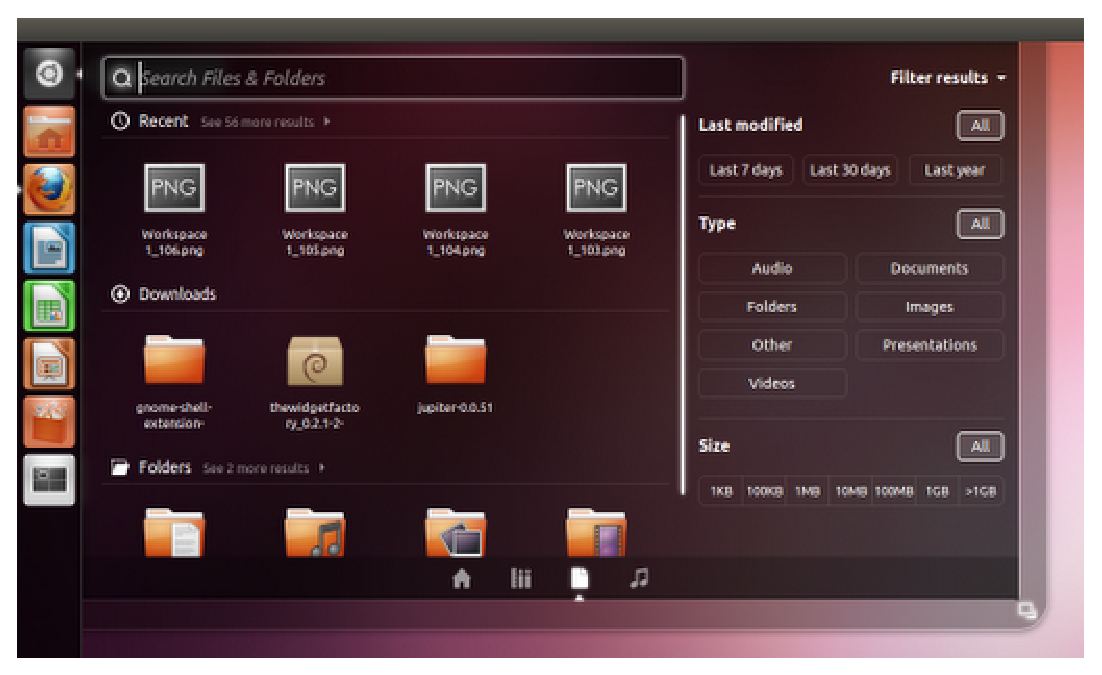
\includegraphics[width=0.5\textwidth]{../images/ubuntugui}
  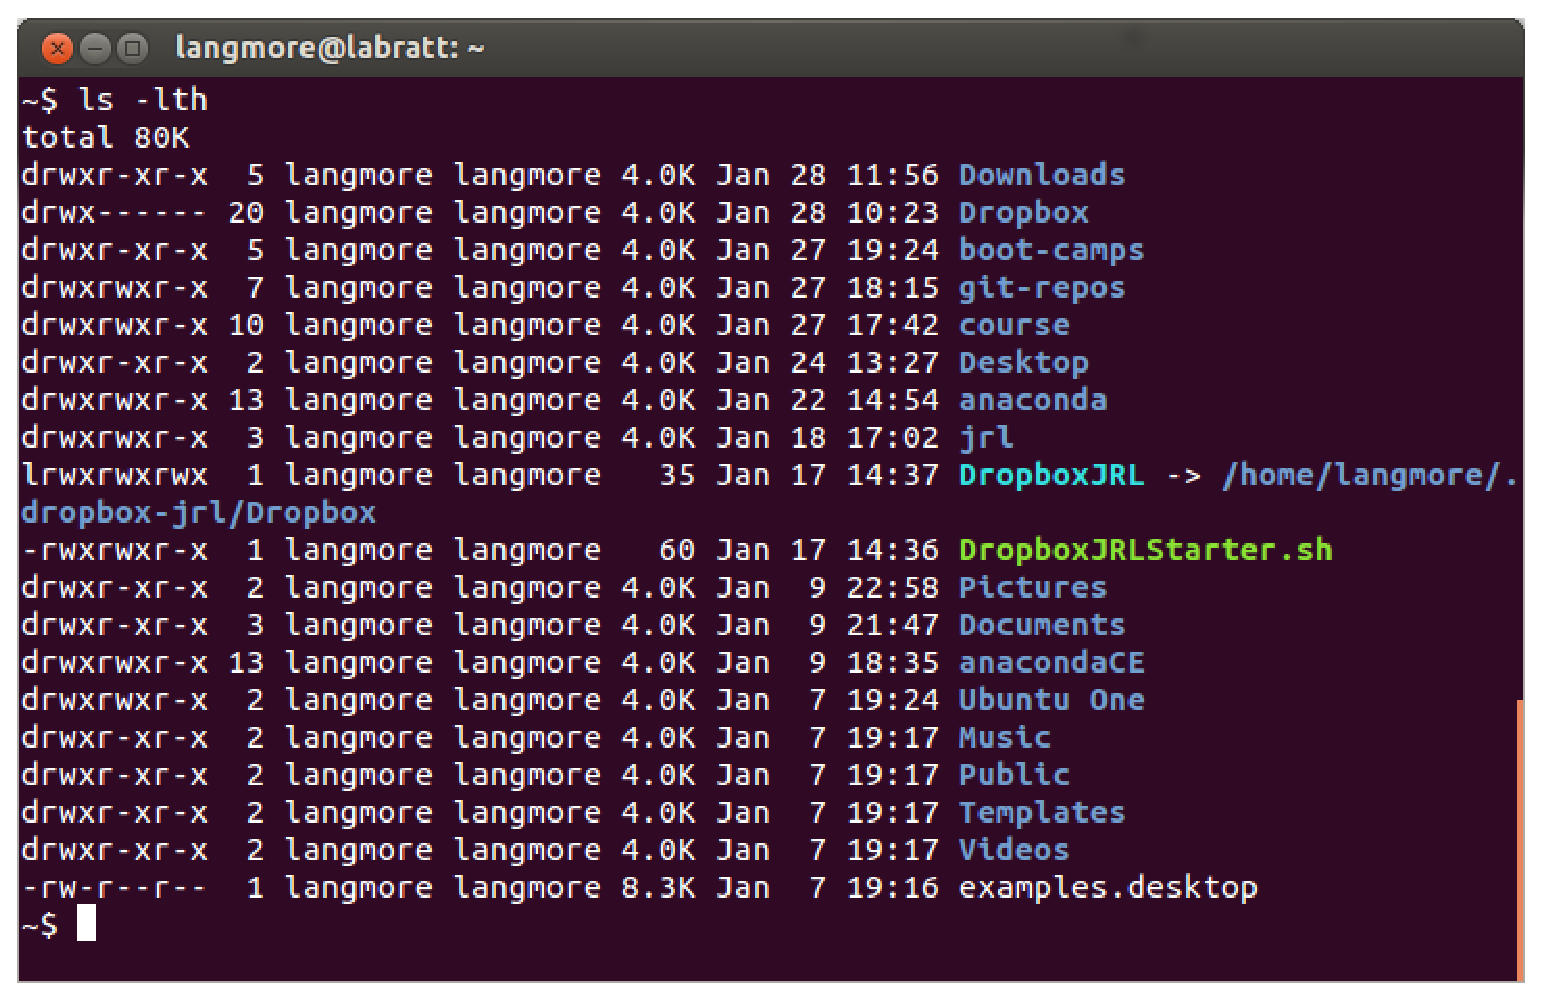
\includegraphics[width=0.5\textwidth]{../images/terminal}
  \caption{Ubuntu's GUI and CLI}
\end{figure}

\begin{digression}[Linux without tears]
  The easiest way to have access to the bash shell and a modern scientific computing environment is to buy hardware that is pre-loaded with Linux.  This way, the hardware vendor is takes responsibility for maintaining the proper drivers.  Use caution when reading blogs talking about how ``easy'' it was to get some off-brand laptop computer working with Linux\ldots this could work for you, or you could be left with a giant headache.  Currently there are a number of hardware vendors that ship machines with Linux:  System76, ZaReason, and Dell (with their ``Project Sputnik'' campaign).  Mac OSX is built on Unix, and also qualifies as a linux machine of sorts.  The disadvantage (of a mac) is price, and the fact that the package management system (for installing software) that comes with Ubuntu linux is the cleanest, easiest ever!
\end{digression}

The shell allows you to control your computer using commands entered in a keyboard.  This sort of interaction is called a \emph{command line interface} (CLI).  ``The shell'' in our case will refer to the \emph{Bourne again} or \emph{bash shell}.  The bash shell provides an interface to your computer's OS along with a number of utilties and minilanguages.  We will introduce you to the shell during the software carpentry bootcamp.  For those unable to attend, we refer you to
% TODO Insert reference

Why learn the shell?
\begin{itemize}
  \item The shell provides a number of utilities that allow you to perform tasks such as interact with your OS or modify a text file.
  \item The shell provides a number \emph{minilanguages} that allow you to automate these tasks.
  \item Often programs must communicate with a user or another machine.  A CLI is a very simple way to do this.  Trust me, you don't want to create a GUI for every script you write.
  \item Usually the only way to communicate with a remote computer/cluster is using a shell.
\end{itemize}

Because of this, programs and workflows that \emph{only} work in the shell are common.  For this reason alone, a modern scientist must learn to use the shell.

Shell utilities have a common format that is almost always adhered to.  This format is:  \T{utilityname  options  arguments}.  The \emph{utilityname} is the name of the utility, such as \T{cut}, which picks out a column of a csv file.  The \emph{options} modify the behavior of the program.  In the case of \T{cut} this could mean specifying how the file is delimited (tabs, spaces, commas, etc\ldots) and which column to pick out.  In general, options should in fact be \emph{optional} in that the utility will work without them (but may not give the desired behavior).  The \emph{arguments} come last.  These are not optional and can often be thought of as the external input to the program.  In the case of \T{cut} this is the file from which to extract a column.  Putting this together, if \T{data.csv} looks like:
\begin{minted}{bash}
  name,age,weight
  ian,1,11
  chang,2,22
\end{minted}
Then
\begin{align}
  &\underbrace{\T{cut}}_\text{utilityname}  \underbrace{\T{-d, -f1}}_\text{options}\quad \underbrace{\T{data.csv}}_\text{arguments}
  \label{unix:align:cut}
\end{align}
produces (more specifically, prints on the terminal screen)
\begin{minted}{bash}
  age
  1
  2
\end{minted}

\section{Streams}
A \emph{stream} is general term for a sequence of data elements made available over time.  This data is processed one element at a time.  For example, consider the data file (which we will call \T{data.csv}):
\begin{minted}{bash}
  name,age,weight
  ian,1,11
  chang,2,22
  daniel,3,33
\end{minted}
This data may exist in one contiguous block in memory/disk or not.  In either case, to process this data as a stream, you should view it as a contiguous block that looks like
\begin{minted}{bash}
  name,age,weight\n ian,1,11\n chang,2,22\n daniel,3,33
\end{minted}
The special character \lstinline$\n$ is called a \emph{newline} character and represents the start of a new line.  The command \T{cut -d, -f2 data.csv} will pick out the second column of \T{data.csv}, in other words, it returns
\begin{minted}{bash}
  age
  1
  2
  3
\end{minted}
, or, thought of as a stream,
\begin{minted}{bash}
  age\n 1\n 2\n 3
\end{minted}
This could be accomplished by reading the file in sequence, starting to store the characters in a buffer once the first comma is hit, then printing when the second comma is hit.  Since the newline is such a special character, many languages provide some means for the user to process each line as a separate item.

This is a very simple way to think about data processing.  This simplicity is advantageous and allows one to scale stream processing to massive scales.  Indeed, the popular Hadoop MapReduce implementation requires that all small tasks operate on streams.  Another advantage of stream processing is that memory needs are reduced.  Programs that are able to read from stdin and write to stdout are known as \emph{filters}.

\subsection{Standard streams}
While stream is a general term, there are three streaming input and output channels available on (almost) every machine.  These are \emph{standard input} (stdin), \emph{standard output} (stdout), and \emph{standard error} (stderr).  Together, these \emph{standard streams} provide a means for a \emph{process} to communicate with other processes, or a computer to communicate with other machines (see figure \ref{unix:fig:stdstreams}).  Standard input is used to allow a process to read data from another source.  A Python programmer could read from standard in, then print the same thing to standard out using
\begin{minted}{python}
for line in sys.stdin:
    sys.stdout.write(line)
\end{minted}
If data is flowing into stdin, then this will result in the same data being written to stdout.  If you launch a terminal, then stdout is (by default) connected to your terminal display.  So if a program sends something to stdout it is displayed on your terminal.  By default stdin is connected to your keyboard.  Stderr operates sort of like stdout but all information carries the special tag, ``this is an error message.''  Stderr is therefore used for printing error/debugging information.
\begin{figure}
  \label{unix:fig:stdstreams}
  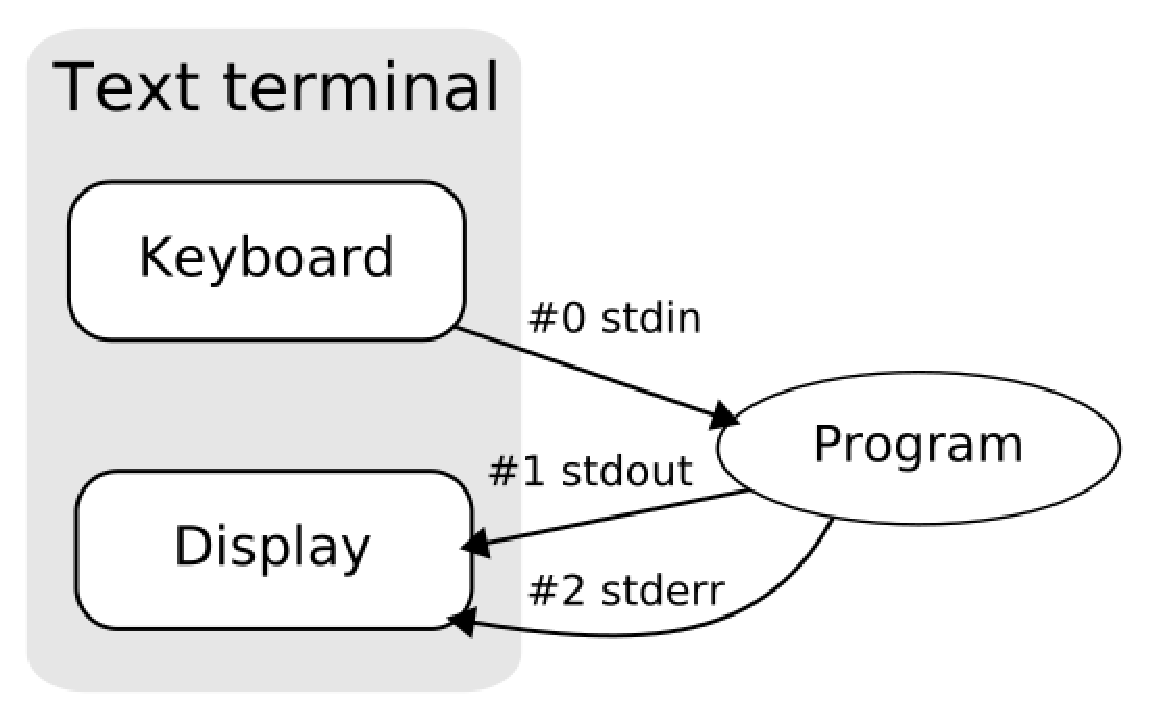
\includegraphics[width=0.7\textwidth]{../images/Stdstreams-notitle}
  \caption{Illustration of the standard streams}
\end{figure}


\subsection{Pipes}
\label{subsection:pipes}
The standard streams aren't any good if there isn't any way to access them.  Unix provides a very simple means to connect the standard output of one process to the standard input of another.  This construct called a \emph{pipe} and is written with a vertical bar \T{|}.  Utilities tied together with pipes form what is known as a \emph{pipeline}.

Consider the following pipeline
\begin{minted}{bash}
  \$ cat infile.csv | cut -d, -f1 | sort | uniq -c
\end{minted}
The above line reads in a text file and prints it to standard out with \T{cat}, the pipe ``\textbar'' redirects this standard out to the standard in of \T{cut}.  \T{cut} in turn extracts the first column and passes the result to \T{sort}, which sends its result to \T{uniq}.  \T{uniq -c} counts the number of unique occurrences of each word.

Let's decompose this step-by-step:  First, print \emph{infile.csv} to stdout (which is, by default, the terminal) using cat.
\begin{minted}{bash}
  \$ cat infile.csv

  ian,1
  daniel,2
  chang,3
  ian,11
\end{minted}
Second, pipe this to \T{cut}, which will extract the first \emph{field} (the \T{-f} option) in this comma delimited (the \T{-d,} option) file. 
\begin{minted}{bash}
  \$ cat infile.csv | cut -d, -f1

  ian
  daniel
  chang
  ian
\end{minted}
Third, pipe the output of cut to sort
\begin{minted}{bash}
  \$ cat infile.csv | cut -d, -f1 | sort

  chang
  daniel
  ian
  ian
\end{minted}
Third, redirect the output of sort to uniq.
\begin{minted}{bash}
  \$ cat infile.csv | cut -d, -f1 | sort | uniq -c

  1  chang
  1  daniel
  2  ian
\end{minted}
It is important to note that uniq counts unique occurrences in consecutive lines of text.  If we did not sort the input to uniq, we would have
\begin{minted}{bash}
  \$ cat infile.csv | cut -d, -f1 | uniq -c

  1  ian
  1  daniel
  1  chang
  1  ian
\end{minted}
\T{uniq} processes text streams character-by-character and does not have the ability to look ahead and see that ``ian'' will occur a second time.


\section{Text}
One surprising thing to some Unix newcomers is the degree to which simple plain text dominates.  The preferred file format for most data files and streams is just plain text.  

Why not use a compressed binary format that would be quicker to read/write using a special reader application?  The reason is in the question:  A special reader application would be needed.  As time goes on, many data formats and reader applications come in, and then out of favor.  Soon your special format data file needs a hard to find application to read it\footnote{Any user of Microsoft Word documents from the 90's should be familiar with the headaches that can arise from this situation.}.  What about for communication between processes on a machine?  The same situation arises:  As soon as more than one binary format is used, it is possible for one of them to become obsolete.  Even if both are well supported, every process needs to specify what format it is using.  Another advantage of working with text streams is the fact that humans can visually inspect them for debugging purposes.

While binary formats live and die on a quick (computer) time-scale, change in human languages changes on the scale of at least a generation.  In fact, one summary of the Unix philosophy goes, ``This is the Unix philosophy: Write programs that do one thing and do it well. Write programs to work together. Write programs to handle text streams, because that is a universal interface.''

This, in addition to the fact that programming in general requires manipulation of text files, means that you are required to master decent text processing software.  Here is a brief overview of some popular programs
\begin{itemize}
  \item {\bf Vim} is a powerful text editor designed to allow quick editing of files and minimal hand movement.
  \item {\bf Emacs} is another powerful text editor.  Some people find that it requires users to contort their hands and leads to wrist problems.
  \item {\bf Gedit, sublime text} are decent text editors available for Linux and Mac.  They are not as powerful as Vim/Emacs, but don't require any special skills to use.
  \item {\bf nano} is a simple unix text editor available on any system.  If nano doesn't work, try \emph{pico}.
  \item {\bf sed} is a text stream processing command line utility available in your shell.  It can do simple operations on one line of text at a time.  It is useful because of its speed, and the fact that it can handle arbitrarily large files.
  \item {\bf awk} is an old school minilanguage that allows more complex operations than sed.  It is often acknowledged that awk syntax is too complex and that learning to write simple Python scripts is a better game plan.
\end{itemize}
\section{Philosophy}
The Unix culture carries with it a philosophy about software design.  The Unix operating system (and its core utilities) can be seen as examples of this.    Let's go over some key rules.  With the exception of the rule of collaboration, these appeared previously in \cite{RaymondUnix}.

\subsection{In a nutshell}

\vspace{0.1in}
\noindent\textit{\textbf{Rule of Simplicity.}}
Design for simplicity.  Add complexity only when you must.

\vspace{0.1in}
\noindent\textit{\textbf{Rule of Collaboration.}}
Make programs that work together.  Work together with people to make programs

\subsection{More nuts and bolts}

We can add more rules to the two main rules above, and provide hints as to how they will guide our software development.  Our programs will be small, so (hopefully) few compromises will have to be made.

\textit{\textbf{Rule of Simplicity.}}
This is sometimes expressed as K.I.S.S, or ``Keep It Simple Stupid.''  All other philosophical points presented here can be seen as special cases of this.  Complex programs are difficult to debug, implement, maintain, or extend.  We will keep things simple by, for example:
(i) writing CLI utilities that \emph{do one thing well},
(ii) avoiding objects unless using them results in a simpler, more transparent design,
and
(iii) in our modules, include only features that will be used right now.

\textit{\textbf{Rule of Collaboration.}}
We will make programs that work together by, for example:
(i) writing CLI utilities that work as filters,
and
(ii) choosing common data structures (such as Numpy arrays, Pandas DataFrames).
We will work together with people to make programs by, for example:
(i) employing Git as a version control system (using Github to host our code)
and,
(ii) enforcing code readability standards such as PEP8.

\textit{\textbf{Rule of Modularity.}}
Write simple parts connected by clean interfaces.  Humans can hold only a limited amount of information in their head at one time.  Make your functions small (simple) enough so that they can be explained in one sentence.

\textit{\textbf{Rule of Clarity.}}
Clarity is better than cleverness.  Maintenance and debugging of code is very expensive.  Take time to make sure your program logic will be clear to someone reading your code some time in the future (this person might be you).  Comments are important.  Better yet, code can often be written to read like a story\dots and no comments are necessary.
\begin{minted}{python}
  for row in reader:
      rowsum = sum_row(row)
      row.append(rowsum)
      writer.write(row)
\end{minted}

\textit{\textbf{Rule of Composition.}}
Design programs to be connected to other programs.  The Unix command line utilities are an example of this.  They (typically) can read from a file or stdin, and write to stdout.  Thus, multiple utilities can be tied together with pipes.
\begin{minted}{bash}
  cat infile.csv | cut -f1 | sort | uniq -c
\end{minted}


\textit{\textbf{Rule of Least Surprise.}}
Try to do the least surprising thing.  We will follow Unix or Python convention whenever possible.  For example, our data files will be in common formats such as csv, xml, json, etc\dots


\section{End Notes}
\emph{Revolution OS} is a fun movie about the rise of Linux.

\cite{RaymondUnix} gives a comprehensive exposition of the history and philosophy of Unix, and provides most of the material you see in our history and philosophy sections.  

The quote by Kernighan and Pike can be found in ``The Unix programming environment.''\cite{UnixProgrammingEnvironment}

Software Carpentry held a bootcamp for students in three courses at Columbia University in 2013 \cite{SWC-NYC2013}.

The impact of the inventions to come out of Bell Labs cannot be understated.  Also developed there were radio astronomy, the transistor, the laser, the CCD, information theory, and the C/C++ programming languages.\cite{BellLabsWikipedia}
